\documentclass[10pt, a4paper]{jsarticle}
\title{モンテカルロ木探索における\\シミュレーションのGPUを用いた並列化}
\author{明治大学理工学部情報科学科\\知的情報処理システム研究室\\4年15組28番 高野昂平}
\date{}

\usepackage[dvipdfmx]{graphicx}

\begin{document}
\maketitle
\tableofcontents
\newpage
\section{はじめに}
\subsection{研究概要}
モンテカルロ木探索(Monte Carlo Tree Search, MCTS)におけるシミュレーション部分を並列化し、高速化を目指す。
オセロを対象に実験を行った。
\subsection{研究背景}
モンテカルロ木探索の処理速度向上を図るうえで、シミュレーション部分が全体の処理速度のボトルネックとなっているのではと考え、シミュレーション部分を並列化することが全体の高速化につながるのではないかと考えた。\par
高性能なCPUを用いることで高速化を図ることも考えられるが、近年CPUの性能向上率が以前に比べて伸び悩んでおり、高速化を図るためにはCPUに依存した手法では高止まりになってしまう。そこで、別のアプローチで高速化を目指す必要があるが、その手法としてGPUを用いた並列化を選択した。近年、GPUを画像処理だけでなく、汎用計算に用いてGPGPU(Generarl Purpose GPU)として活用する動きも見られるため、モンテカルロ木探索に対してもGPGPUとして活用できないものかと考えた。
\section{関連研究}
\section{モンテカルロ木探索について}
本研究のテーマであるモンテカルロ木探索(Monte Carlo Tree Search, MCTS)とは、乱数を用いた計算手法であるモンテカルロ法を木探索に応用した手法である。\par
まず、評価関数を用いないという特徴を持つため、様々なゲームのプレイヤーに対してモンテカルロ木探索を実装することができる。例えば、General Game Playing(GGP)という汎用ゲームに対して人間の介入なしで強いプレイヤーを作るという試みがあるが、そのプレイヤーとしてモンテカルロ木探索を用いることが可能である。\par
また、不要な探索を行わないという特徴を持つ。合法手が膨大なゲームに対して木探索を行う場合、そのすべてのノードを探索することによって強いプレイヤーの作成するのは計算量が多くなってしまい、現実的でない。例えば、本研究ではオセロのプレイヤーに対して、モンテカルロ木探索を施したが、そのオセロの合法手は$10^{28}$手あると推測されており、すべてのノードを探索することが困難であることがわかる。しかし、モンテカルロ木探索の場合、すべてのノードを探索するのではなく、有効と考えられる手を優先的に深く探索するため、無駄な探索をすることがなく、計算量を削減することができる。\par
モンテカルロ木探索の流れとしては、選択、シミュレーション、展開、逆伝播の4ステップからなっており(図1)、本研究では2ステップ目のシミュレーションを並列化することを目標としている。
\subsection{UCTについて}
選択ステップにおいて、次に訪問するノードを決めるアルゴリズムとして、UCTアルゴリズムを採用した。このアルゴリズムは、以下の式が最大となるようなノードを次の訪問ノードとするアルゴリズムである。\par
以下の式において、$w$はそのノードにおける評価値、$n$はそのノードにおける訪問回数、$N$はそのノードを親としたと きの子ノードの$n$の値の合計値、$C$は任意の値で探索がうまくいくように調整すべきパラメータとなっている。
\begin{eqnarray}
    UCT = \frac{w}{n} + C\sqrt{\frac{\ln{N}}{n}}
\end{eqnarray}
\par
この式が意味するのは、ノードの評価値だけで訪問先を決めるのではないということで、第1項自体は評価値の平均を取っているが、第2項において訪問回数が少ないノードを訪問するようにUCT値を調整しているのがわかる。変数$C$はこの訪問回数の少ないノードへの訪問をどれくらい重く見るべきか定めるパラメータと言える。
\subsection{並列化手法}
本研究では、シミュレーション部分を並列化するが、具体的には以下の図1のように、4ステップあるモンテカルロ木探索の2ステップ目を複数回のシミュレーションを同時に実行することで実現する。
\begin{figure}[h]
    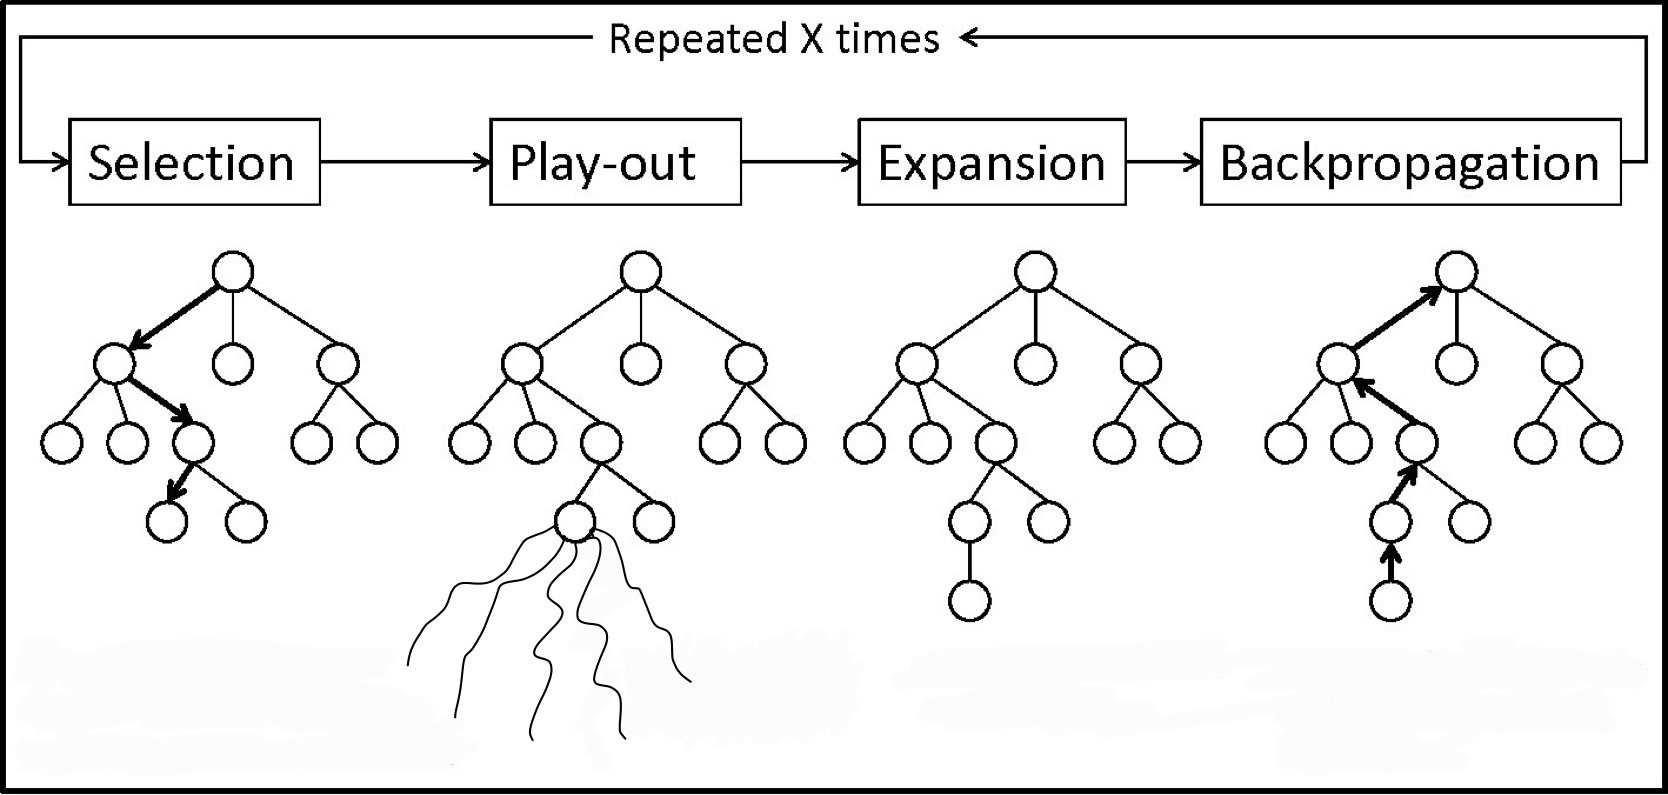
\includegraphics[width=15cm]{img/mcts_parallel.jpg}
    \caption{シミュレーションの並列化}
\end{figure}
\par
並列化にあたって、NVIDIA社のCUDA(Compute Unified Device Architecture)を用いた。CUDAはNVIDIA社のGPU上で動作する汎用並列コンピューティングプラットフォームである。なお、言語はC++とし、CUDA Cを用いて実装を行った。
\section{実験}
\subsection{パラメータについて}
\subsection{実行環境}
CUDAを用いる関係上、GPUはNVIDIA社のものとなっている。
\begin{table}[h]
    \begin{center}
        \begin{tabular}{ll}
            OS & Ubuntu 20.04.2 LTS \\
            CPU & Intel(R) Core(TM) i9-10900X CPU @ 3.70GHz \\
            GPU & GeForce RTX 3080 \\
            メモリ & 32GB \\
        \end{tabular}
    \end{center}
\end{table}
\section{終わりに}
\end{document}